\section{Sinusoidal Analysis and Modelling}

\subsection{Introduction}

Different musical applications need the \textbf{analysis} of a sound, and with that the definition of sinusoidal analysis.
In order to understand the frequency content of a sound, we define a frequency transformation using the \textbf{Short Time Fourier Transform} (STFT, frequency domain) or by \textbf{filterbanks} (time domain).

\begin{figure}[H]
    \centering
    
\includegraphics[width=0.5\linewidth]{STFT.png}
    \caption{STFT by windowing $ x(t) $ and applying FFT for each frame}
\end{figure}

An important aspect of audio analysis is to track the presence of certain frequencies along the entire spectrum, along the entire sound duration.
An example of peak detection application is automatic music transcription, where we first need to convert the audio track into a time-frequency representation (like a chromagram).
That is similar to what happens in forensic analysis, when searching for audio recordings into electrical networks.

\begin{figure}[H]
    \centering
    \begin{minipage}{0.25\linewidth}
        \centering
        
\includegraphics[width=\linewidth]{Automatic transcription.png}
    \end{minipage}
    \hspace{0.4cm}
    \begin{minipage}{0.5\linewidth}
        \centering
        
\includegraphics[width=\linewidth]{Electric network.png}
    \end{minipage}
    \caption{Automatic music transcription (left), electrical network analysis (right)}
\end{figure}

After switching from time to frequency domain for audio analysis, we can \textbf{synthesize} the track back again into time domain, through \textbf{Inverse-STFT} (frequency domain) or with a \textbf{bank of oscillators} (time domain).

Note that it is easier to implement analysis and synthesis in the same domain (time or frequency), rather than changing domain in between.

\begin{figure}[H]
    \centering
    
\includegraphics[width=0.4\linewidth]{Analysis_synthesis.png}
    \caption{Analysis-synthesis schematic}
\end{figure}

Other music applications requires synthesized audio, such as frequency-domain elaborations.
Other applications, on the other hand, exploit both analysis and synthesis, like a data-compressed audio representation that allows easy implementation of different audio transformations.

The overall \textbf{analysis-synthesis pipeline} consists in:

\begin{itemize}
    \item \textbf{Analysis}: STFT or filterbank
    \item \textbf{Data reduction} (optional)
    \item \textbf{Modification} (optional)
    \item \textbf{Synthesis}: Inverse-STFT or bank of oscillators
\end{itemize}

\subsection{Resolving sinusoidal peaks}

\subsubsection{Spectral analysis}

Let us consider a time signal $ s_s(t) $ to analyse, which can be well approximated by a sum of sinusoids:

\[
s_s(t) = \sum_k a_k(t) \cos(\varphi_k(t))
\]

We want to determine how many sinusoids are present and their parameters (frequency $f$, amplitude $a$, phase $\varphi$).
Note that, differently from a \textbf{Fourier series}, the amplitude terms $a_k(t)$ are not constant, but time-varying.
The presented approximation is called \textbf{instantaneous sinusoidal model}.

\subsubsection{Windowing effect}

Let us now understand a \textbf{practical difficulty}: real signals are finite in time, like they are a \textbf{windowed} version of an infinite signal.
The frequency detection of an infinite sinusoid is trivial:

\begin{figure}[H]
    \centering
    
\includegraphics[width=0.3\linewidth]{Sinusoid.png}
    
\includegraphics[width=0.36\linewidth]{Sinusoid FT.png}
    \caption{Sinusoid $ x(n) = e^{j \omega_0 nT} $ and its Fourier transform $ X(\omega) = \delta (\omega - \omega_0) $}
\end{figure}

\clearpage

A windowed signal transformation, on the other hand, suffers from \textbf{sidelobes}:

\begin{figure}[H]
    \centering
    
\includegraphics[width=0.3\linewidth]{Windowed sinusoid.png}
    
\includegraphics[width=0.36\linewidth]{Windowed ft.png}
    \caption{Windowed $ x(n) = w(n) \ e^{j \omega_0 nT} $ and its Fourier transform $ X(\omega) = W(\omega) * \delta (\omega - \omega_0) $}
\end{figure}

The presence of many sidelobes can make it difficult to \textbf{detect the real peaks} of the audio signal.
For example, when \textbf{two sinusoids} are combined, the resulting Fourier transform may or not be able to detect two separate frequencies:

\begin{figure}[H]
     \centering
     
\includegraphics[width=0.95\linewidth]{Windows length.png}
     \caption{Window's length $M$ effect on Fourier transform and peak detection of two combined sinusoids}
\end{figure}

Not only the window's length, but its type influences the analysis as well:

\begin{figure}[H]
     \centering
     
\includegraphics[width=0.6\linewidth]{Windows effect.png}
     \caption{Windows sidelobes height (left) and windows shape (right)}
\end{figure}

We may notice that there is a trade-off between mainlobe width and sidelobes height:

\begin{table}[H]
    \centering
    \begin{tabular}{cccc}
        %\hline
        \toprule
        Window type & Peak sidelobe amplitude (dB) & Mainlobe width & Roll off \\ [3pt]
        % \hline \hline
        \midrule
        Rectangular & -13 & $ \frac{4\pi}{M-1} \approx 2\Omega_M $ & 6 dB/oct \\ [3pt]
        % \hline
        Bartlett $\Delta$ & -25 & $ \frac{8\pi}{M} = 4\Omega_M $ & 12 dB/oct \\ [3pt]
        % \hline
        Hann & -31 & $ \frac{8\pi}{M} = 4\Omega_M $ & 18 dB/oct \\ [3pt]
        % \hline
        Hamming & -41 & $ \frac{8\pi}{M} = 4\Omega_M $ & 6 dB/oct (after first sidelobe) \\ [3pt]
        % \hline
        Blackman & -58 & $ \frac{12\pi}{M} = 6\Omega_M $ & 18 dB/oct \\
        \bottomrule
    \end{tabular}
    \caption{Window choice}
\end{table}

The term roll off describes the slope with which the sidelobes amplitude (in dB) decreases (in dB over octave): the higher the roll off value, the faster the sidelobes height decreases, making them negligible in the sound analysis.

\subsubsection{Window length $M$ and frequency resolution $\Delta$}

In order to have a minimum \textbf{resolution requirement}, let's imagine we have two sinusoids with frequency difference $ \Delta $ (in Hz) and we need to distinguish them in the frequency domain.
With the Fourier transform, we obtain two mainlobes for each sinusoid, and we want to avoid overlapping.

\begin{figure}[H]
    \centering
    
\includegraphics[width=0.4\linewidth]{Frequency resolution.png}
    \caption{Frequency resolution $\Delta$ in sinusoidal analysis}
\end{figure}

By considering the desired \textbf{frequency resolution} $\Delta$ and \textbf{mainlobes bandwidth} $B_W$, the requirement becomes:

\[ B_W \leq \Delta = f_2 - f_1 \]

The bandwidth $B_W$ depends on the window parameter $L$, on the sampling frequency $F_s$ (in Hz) and on the \textbf{window length} $M$ (in samples):

\[ B_W = L \frac{F_s}{M} \quad \Rightarrow \quad L \frac{F_s}{M} \leq \Delta \quad \Rightarrow \quad M \geq L \frac{F_s}{\Delta} \quad \Rightarrow \quad M \geq L \frac{F_s}{f_2 - f_1} \]

\begin{figure}[H]
    \centering
    
\includegraphics[width=0.4\linewidth]{Spectogram harmonic instruments.png}
    \caption{Spectrogram of harmonic (top) and non-harmonic (bottom) instruments}
\end{figure}

Many audio signals can be harmonic in nature, with a \textbf{fundamental frequency} $ f_0 $: the minimum frequency separation between the harmonic components will be $ \Delta = f_0 $.

\[ M \geq L \frac{F_s}{\Delta} \quad \Rightarrow \quad M \geq L \frac{F_s}{f_0} \]

We define $ P $ as the \textbf{fundamental period} (in samples) of the signal (sampling period $T_s$):

\[ P = \frac{T_0}{T_s} = \frac{1/f_0}{1/F_s} = \frac{F_s}{f_0} \quad \Rightarrow \quad M \geq LP \]

In order to fully resolve an harmonic sound (with period of $P$ samples), we need windows that cover at least 2 periods with rectangular window ($L=2$), 4 periods with Hamming window ($L=4$), 6 periods with Blackman window ($L=6$), and so on.

For example, let us consider two singers (male and female) with respective fundamental frequency of 100 an 200 Hz.
Using sampling frequency of 50 kHz, the necessary window length $ M $ in samples to resolve correctly is:

\begin{table}[H]
    \centering
    \begin{tabular}{lcc}
        %\hline
        \toprule
         & Male voice ($f_0 = 100$ Hz) & Female voice ($f_0 = 200$ Hz) \\ [3pt]
        % \hline \hline
        \midrule
        Rectangular (L = 2) & $ M \geq L \frac{F_s}{f_0} = 1000 $ & $ M \geq L \frac{F_s}{f_0} = 500 $ \\ [3pt]
        % \hline
        Hamming, Hann (L = 4) & $ M \geq L \frac{F_s}{f_0} = 2000 $ & $ M \geq L \frac{F_s}{f_0} = 1000 $ \\ [3pt]
        % \hline
        Blackman (L = 6) & $ M \geq L \frac{F_s}{f_0} = 3000 $ & $ M \geq L \frac{F_s}{f_0} = 1500 $ \\
        \bottomrule
    \end{tabular}
    \caption{Window minimum length $M$ to separate two voices fundamentals ($\Delta = 100$ Hz, $F_s=50$ kHz)}
\end{table}

To summarize, in order to correctly analyse an audio track (well approximated as sum of time-varying sinusoids) we need a \textbf{sufficiently long window}: its length $M$ is computed knowing the desired frequency resolution $\Delta$, the window type (by means of the window factor $L$) and the sampling frequency $F_s$.

\subsection{Spectral interpolation}

The analysis process consists in detecting correctly the frequency components of an audio.
The synthesis, on the other hand, consists in reconstructing correctly a sinusoidal (or more), starting from the spectrum samples.

\begin{figure}[H]
    \centering
    
\includegraphics[width=0.55\linewidth]{Interpolation.png}
    \caption{Linear interpolation of a Discrete Fourier Transform (DFT) in module $ \abs{X(f)} $}
\end{figure}

In this case, we want a \textbf{localization accuracy} requirement on the samples of the DFT: we may achieve that through \textbf{zero padding} (ideal interpolation, in time domain) or by \textbf{parabolic interpolation}.

\subsubsection{Zero padding}

\textbf{Zero padding} consists in adding zeros after the (windowed) audio signal (in time) and it corresponds to frequency-domain interpolation:

\begin{figure}[H]
    \centering
    
\includegraphics[width=0.55\linewidth]{Zero padding.png}
    \caption{Effect of zero padding (in time) on the DFT resolution (in frequency) with different oversampling factors}
\end{figure}

The \textbf{oversampling factor} of the zero padding indicates how much longer is the new signal in relation to the original version.
By adding zeros through this technique, the DFT has more samples and it becomes more clear, decreasing the chances of error in the interpolation.

For sinusoidal peak detection, spectral interpolation via zero-padding gets us closer to the true maximum of the main lobe when we simply take the maximum-magnitude FFT-bin as our estimate, considering that zero-padding adds more samples to evaluate.

Let us notice that zero padding cannot solve the problem of frequency resolution in the analysis: it is still able to correctly reconstruct the Fourier transform, but the DFT itself is the result of an incorrect analysis (two mainlobes mixed into one).

\begin{figure}[H]
    \centering
    
\includegraphics[width=0.45\linewidth]{Resolution and accuracy.png}
    
\includegraphics[width=0.45\linewidth]{Resolution and accuracy 2.png}
    \caption{Spectrum peak detection with different oversampling factors: successful (left) and unsuccessful frequency resolution (right)}
\end{figure}

Considering a DFT with $ N $ samples, the \textbf{peak localization error} $ \Delta f $ is half a distance between two consecutive samples:

\[ \Delta f = \pm \frac{1}{2} \frac{F_s}{N} = \pm \frac{F_s}{2N} \]

For example, let's consider again the example of the two singers.
Using $M=1024$ samples for the male voice DFT ($F_s=$ 50 kHz), its localization error becomes $ \pm $ 25 Hz, which is 25\% of the fundamental frequency ($ f_0 = $ 100 Hz).
Such a case is not acceptable: we need to zero pad the audio track, increasing its length from $M$ samples (window length) to a way larger $N$ (DFT length).

We remind that the number of samples of the window (in time) is always equivalent to the number of samples of the DFT (in frequency).

The localization requirement for \textbf{spectral interpolation} consists in determining the \textbf{minimum DFT length} $N$ for a correct frequency peak detection.
The minimum frequency difference we want to detect must be less than the Just Noticeable Difference (JND):

\[
\Delta f \leq \text{JND},
\qquad
\text{JND} =
\begin{cases}
     0.5\% \ f, & f \leq 600 \text{ Hz} \\
    3 \text{ Hz}, & f > 600 \text{ Hz}
\end{cases}
\]

In this example, the oversampling factor should be more than 8 (from 1024 to 8333), which means that the zero padding should make the time signal more than 8 times longer:

\[ \frac{F_s}{2N} \leq \text{JND} \quad \Rightarrow \quad N \geq \frac{F_s}{2 \ \text{JND}} = \frac{50 \cdot 10^{3}}{2 \cdot 3} \quad \Rightarrow \quad N \geq 8333, \quad \text{oversampling factor}: \lceil \frac{8333}{1024} \rceil = 9 \]

\subsubsection{Parabolic interpolation}

Zero padding in the time domain results in sinc interpolation in the frequency domain, but other interpolation forms may be used: one of those is the \textbf{parabolic interpolation}, which is particularly effective.
The reason is that, generally, the mainlobe of a DFT is well approximated by an upside-down parabola.
The only exception is when using a Gaussian window (on dB scale), in which case the \textbf{quadratic interpolation} results better.

\begin{figure}[H]
    \centering
    
\includegraphics[width=0.6\linewidth]{Parabola interpolation.png}
    \caption{DFT amplitude (in dB) and parabolic interpolation}
\end{figure}

Given the DFT samples in (-1, $ \alpha $), (0, $ \beta $) and (1, $ \gamma $), the \textbf{best parabola} that interpolates those points is obtained using the parabola formula for each point:

\[ y(x) = a (x-p)^2 + b \]

\begin{figure}[H]
    \centering
    
\includegraphics[width=0.55\linewidth]{Parabola.png}
    \caption{Best parabola parameters identification}
\end{figure}

\[
\left\{
\begin{array}{ccl}
    y(-1) = \alpha & = & a (-1-p)^2 + b = a (1 + p^2 + 2p) + b = ap^2 + 2ap + a + b \\
    y(0) = \beta & = & a (-p)^2 + b = ap^2 + b \\
    y(1) = \gamma & = & a (1-p)^2 + b = a (1 + p^2 - 2p) + b = ap^2 - 2ap + a + b
\end{array}
\right.
\]

\[ \alpha - \gamma = 4ap \quad \Rightarrow \quad p = \frac{\alpha - \gamma}{4a}, \qquad \alpha = ap^2 + \left(\frac{\alpha - \gamma}{2}\right) + a + \left(\beta - ap^2\right) \quad \Rightarrow \quad a = \frac{1}{2} \left(\alpha -2\beta + \gamma\right) \]

The resulting \textbf{peak location} is $ p \in \left[-\dfrac{1}{2}, +\dfrac{1}{2}\right] $ (samples) away from the highest sample (located in $p=0$):

\[ p = \frac{1}{2} \frac{\alpha - \gamma}{\alpha - 2\beta + \gamma} \quad \Rightarrow \quad y(p) = \beta - \frac{1}{4} (\alpha - \gamma) p \]

Let us notice that we only used the \textbf{spectral magnitude} $\abs{X(f)}$ to find the peak position $p$, which can be used to interpolate the \textbf{unwrapped phase} $\angle{X(f)}$.
We may interpolate the phase as we want: assuming that no phase peak occurs in $p$, a simple linear interpolation is sufficient (assuming that we have a high number of samples, which means a high enough oversampling factor for zero-padding).

\begin{figure}[H]
    \centering
    
\includegraphics[width=0.45\linewidth]{Parabola approximation.png}
    \caption{Comparison between true lobe and approximating parabola}
\end{figure}

Alternatively, we may interpolate \textbf{real and imaginary part} separately and combine them to obtain the DFT (we remind that $X(f) \in \mathbb{C}$).

\clearpage

\subsection{Additive synthesis technique: STFT-based analysis}

As already said before, one of the \textbf{synthesis techniques} consists in using a bank of oscillators (additive synthesis) and summing different harmonic oscillations to reconstruct an audio track.

\subsubsection{Analysis: Bank of oscillators vs STFT}

Whenever the analysis process is given by the STFT (frequency domain) and the synthesis process is in the time domain, a domain mismatch occurs: the analysis frame rate is insufficient (\textbf{temporal undersampling}) and we need the spectral continuation of the sound (detecting and matching the peaks in frequency, interpolating them and making them drive an oscillator with certain amplitude and frequency).

\subsubsection{Additive synthesis}

The \textbf{additive synthesis} technique with a bank of $ N $ oscillators results in an audio signal as:

\[ y(t) = \sum_{i=1}^N A_i(t) \sin \left[ \omega_i(t) + \phi_i(t) \right], \quad \omega_i(t) = 2 \pi f_i(t) \]

In order to reproduce a specific signal, we need to identify the sinusoidal components (\textbf{sound analysis}), specifically in terms of amplitude and frequency.

\begin{figure}[H]
    \centering
    
\includegraphics[width=0.35\linewidth]{Additive synthesis.png}
    \caption{Additive synthesis with 4 oscillators}
\end{figure}

\subsubsection{Tracking sinusoidal peaks}

What we want to do is to identify the sinusoidal peaks and determine a track (between Fourier transforms of consecutive time frames).
The \textbf{spectral continuation problem} (or better, the sinusoidal tracking in the STFT) arises because we need STFT content in order to define amplitude and frequency for each oscillator in the bank.
This kind of problematic does not occur if the analysis involves filterbanks (dual to the bank of oscillators).

\begin{figure}[H]
    \centering
    
\includegraphics[width=0.5\linewidth]{Sinusoidal tracking.png}
    \caption{Peak tracking: frequency trajectories}
\end{figure}

The STFT-based analysis allows to address some difficulties inherent in vocoders (filterbank-based analysis).
This synthesis technique works for \textbf{both harmonic} and \textbf{inharmonic sounds}, in addition to that the fact that the analysis focuses only near the spectral peaks (instead of fixed filter bands along the entire bandwidth).
The sinusoidal \textbf{parameters estimation} is \textbf{non-coherent}: the phase is discarded, so the magnitude spectrum is sufficient for the synthesis characterization.
In addition to that, separating amplitude and frequency information allows to \textbf{easily implement time-scaling} and \textbf{frequency-shifting} operations (by simply resampling or changing the parameters).

\begin{figure}[H]
    \centering
    
\includegraphics[width=0.75\linewidth]{Analysis system.png}
    \caption{Block diagram of STFT-based analysis system}
\end{figure}

We use quadratic interpolation (in the magnitude spectrum) to identify the spectrum peaks.
Phase is usually discarded for steady-state signals, while it is taken in consideration for audio transient frames.

\begin{figure}[H]
    \centering
    
\includegraphics[width=0.4\linewidth]{Frequency reconstruction.png}
    \caption{Sinusoidal component linear interpolation and reconstruction problem}    
\end{figure}

The frequency peaks of each sinusoidal component should be interconnected frame by frame.
Linear interpolation may be used to define amplitude and frequency of each frequency component when phase is discarded, while cubic interpolation may be used when the phase is retained.

\begin{figure}[H]
    \centering
    
\includegraphics[width=0.4\linewidth]{Peak tracking.png}
    \caption{Possible peak tracking across frames}
\end{figure}

Intuitively speaking, the problem of sinusoidal reconstruction consists in understanding \textbf{"how to connect the dots"}.
Some recommendations may be:

\begin{itemize}
    \item exploit \textbf{harmonicity} whenever possible (even with missing fundamental);
    \item not consider a trajectory dead yet (\textbf{possible gap});
    \item not consider a new trajectory formation yet (\textbf{possible noise}).
\end{itemize}

In other words, the more consistent are the trajectories, the better.
In addition to that, noisy spectra are harder to manage for sure, and a transient detector may be used in order to retain or not the phase.

\subsubsection{Spectral Modelling Synthesis (SMS)}

The synthesis block diagram is given:

\begin{figure}[H]
    \centering
    
\includegraphics[width=0.55\linewidth]{Synthesis system.png}
    \caption{Phase-preserving synthesis system}
\end{figure}

In the \textbf{Spectral Modelling Synthesis} (SMS), the signal spectrum is considered as made up by a \textbf{deterministic component} (sinusoids) and a \textbf{stochastic component} (time-varying noise):

\[ s(t) = \underbrace{\sum_{i=1}^N {A_i(t) \cos[\theta_i(t)]}}_\text{deterministic} + \underbrace{e(t)}_\text{stochastic} \]

By assuming the random component $ e(t) $ as a \textbf{white noise} $ u(t) \sim \mathcal{N} (\mu, \sigma^2) $ \textbf{filtered} by $h_t$:

\[ e(t) = h_t * u(t) = \int_{-\infty}^{+\infty} {h_t(t-\tau) \ u(\tau) \ d\tau} \quad \Rightarrow \quad s(t) = \sum_{i=1}^N {A_i(t) \sin[\omega_i(t) t + \phi_i(t)]} + h_t * u(t) \]

The analysis-synthesis scheme to approximate the stochastic noise $ e(t) $ spectrum is given:

\begin{figure}[H]
    \centering
    
\includegraphics[width=1.0\linewidth]{Analysis and SMS.png}
    \caption{STFT analysis and noise spectrum approximation}
\end{figure}

The synthesis scheme, knowing both the sinusoids trajectories and the noise spectrum, is given:

\begin{figure}[H]
    \centering
    
\includegraphics[width=0.55\linewidth]{Synthesis.png}
    \caption{SMS block diagram}
\end{figure}

\subsection{Additive synthesis technique: filterbank analysis}

When both analysis and synthesis are in time domain, there is no domain mismatch.

The configuration of filterbanks analysis and bank of oscillators synthesis is the first ever obtained (in the late 1930s), even before computers were available, and it is the base of the \textbf{vocoder} (Voice Coder).

Vocoders were initially used for speech coding and transmission, where different elaborations may take place (data compression, noise reduction and reverberation suppression).
Two different versions of vocoders exist: \textbf{channel vocoder} (filterbanks determine the magnitude only) and \textbf{phase vocoder} (filterbanks determine both magnitude and phase).

\begin{figure}[H]
    \centering
    
\includegraphics[width=0.65\linewidth]{Vocoder.png}
    \caption{Vocoder scheme}
\end{figure}

In the vocoder scheme, we divide the signal $x(t)$ into $N$ \textbf{frequency sub-intervals}: from each sub-signal $x_k(t)$ we compute magnitude (and optionally phase) spectrum for further elaborations.

\clearpage

Let us suppose that in each sub-interval (and sub-signal) we have only one sinusoid (that may change over time).
Considering the sub-interval $k$ centered at frequency $\omega_k$, the sub-signal $x_k(t)$ is:

\[ x_k(t) = a_k(t) \cos \left( \omega_k t + \phi_k(t) \right), \qquad a_k(t): \text{amplitude}, \quad \phi_k(t): \text{phase} \]

Amplitude $a_k$ and phase $\phi_k$ terms are all we need to drive the $k$-th oscillator and implement additive synthesis.

\begin{figure}[H]
    \centering
    
\includegraphics[width=0.35\linewidth]{Subband analysis.png}
    
\includegraphics[width=0.2\linewidth]{subband synthesis.png}
    \caption{Sinusoidal parameters for sub-signal $x_k$, analysis (left) and synthesis (right)}
\end{figure}

The phase term includes the instant frequency in terms of \textbf{instant frequency deviation} from $\omega_k$:

\[ \Delta\omega_k(t) = \frac{\partial \phi_k(t)}{\partial t} \]

\subsubsection{Channel vocoder}

The channel vocoder uses the amplitude only: a way to compute it is to apply an \textbf{envelope follower} (to each sub-interval), using a rectifier (module) and a low-pass filter (averaging).

\begin{figure}[H]
    \centering
    
\includegraphics[width=1\linewidth]{Envelope follower.png}
    \caption{Envelope follower and sub-signal amplitude profile}
\end{figure}

The operation is similar to the demodulation of a radio-frequency signal, where the carrier signal is cut from the information signal using an LPF:

\begin{figure}[H]
    \centering
    
\includegraphics[width=0.6\linewidth]{RF demodulation.png}
    \caption{Demodulation of a RF signal}
\end{figure}

\subsubsection{Phase vocoder}

The phase vocoder uses both amplitude and phase of the signal (and sub-signals).
Before discussing the phase vocoder, let us define some \textbf{equivalent representations} of narrow-band signals.

\begin{figure}[H]
    \centering
    
\includegraphics[width=0.45\linewidth]{Narrowband.png}
    
\includegraphics[width=0.45\linewidth]{Analytic signal.png}
    
\includegraphics[width=0.45\linewidth]{Baseband equivalent.png}
    \caption{Narrow-band signal (left), analytic signal (right), baseband equivalent signal (bottom)}
\end{figure}

Let us consider the sub-signal $x_k(t)$ as a \textbf{narrow-band signal} with frequency content around the frequency $f_k$:

\[ x_k(t) = a_k(t) \cos \left( \omega_k t + \phi_k(t) \right) = \frac{a_k}{2} \left[ e^{j\left( \omega_k t + \phi_k(t) \right)} + e^{-j\left( \omega_k t + \phi_k(t) \right)} \right] \]

By selecting the positive-frequency portion of the spectrum with double the amplitude, we define the \textbf{analytic signal}:

\[ x_k^a (t) = a_k(t) \ e^{j\left( \omega_k t + \phi_k(t) \right)}  \]

By demodulating the analytic signal (removing the sub-band frequency $\omega_k$ contribution), we define the \textbf{baseband equivalent signal}:

\[ x_k^m(t) = x_k^a(t) \ e^{-j \omega_k t} = a_k(t) \ e^{j \phi_k(t)} \]

\begin{figure}[H]
    \centering
    \begin{minipage}{0.4\linewidth}
        \centering
        
\includegraphics[width=\linewidth]{Real imaginary analytic.png}
    \end{minipage}
    \hspace{0.4cm}
    \begin{minipage}{0.5\linewidth}
        \centering
        
\includegraphics[width=\linewidth]{Hilbert transformation.png}
    \end{minipage}
    \caption{Real and imaginary part of analytic signal (left) and visualization (right)}
\end{figure}

We want to compute \textbf{real} and \textbf{imaginary part} of the \textbf{analytic signal} in order to define amplitude and phase terms:

\[ a_k(t) = \abs{x_k^a(t)} = \sqrt{\mathrm{Re}(x_k^a(t))^2 + \mathrm{Im}(x_k^a(t))^2}, \qquad \phi_k(t) = \angle{x_k^a(t)} - \omega_k t = \tan^{-1} \left[ \frac{\mathrm{Im}(x_k^a(t))}{\mathrm{Re}(x_k^a(t))} \right] - \omega_k t \]

The real part computation is immediate:

\[ \mathrm{Re}(x_k^a(t)) = x_k(t) \]

While the imaginary part is the result of the \textbf{Hilbert Transform} of $x_k(t)$.
The \textbf{frequency response} (and impulsive response) of the Hilbert transform is:

\[ G_H(f) = -j \ \sign(f) = e^{-j \frac{\pi}{2} \sign(f)} \quad \overset{\mathcal{F}^{-1}}{\longrightarrow} \quad g_H(t) = \frac{1}{\pi t} \]

The closed-form expression for the Hilbert transform $\hat{x}(t)$ of the signal $x(t)$ is the following:

\[ \hat{x}(t) = \int_{-\infty}^{+\infty} x(\tau) \underbrace{\frac{1}{\pi(t-\tau)}}_{g_H(t-\tau)} \ d\tau = \frac{1}{\pi} \int_{-\infty}^{+\infty} \frac{x(\tau)}{t-\tau} \ d\tau \]

We can define the imaginary part of the analytic signal as the Hilbert transform of the narrow-band signal $x_k$:

\[ \mathrm{Im}(x_k^a(t)) = \hat{x}(t) \quad \Rightarrow \quad x_a(t) = x(t) + j \ \hat{x}(t) \]

\[ \mathrm{Im}(x_k^a(t)) \quad \overset{\mathcal{F}}{\longrightarrow} \quad \hat{X}(f) = \frac{1}{2} \left[ X_a(f) - X_a^*(f) \right] = \frac{1}{2j} \left[ 1(f) - 1(-f) \right] X(f) = \underbrace{-j \ \sign(f)}_{G_H(f)} \ X(f) \]

We are able to recover the original signal from the Hilbert transform.
The Hilbert filter is an \textbf{all-pass filter}, so the \textbf{inverse Hilbert filter} exists:

\[
G_{H,I} (f) = \frac{1}{G_H(f)} = j \sign(f) \quad \overset{\mathcal{F}^{-1}}{\longrightarrow} \quad g_{H,I}(t) = -g_H(t) = -\frac{1}{\pi t}
\]

The \textbf{characteristic of the phase vocoder} is the need of computing the phase: we are now able to do that thanks to the identification of real and imaginary part of the analytic signal.
We remind the \textbf{phase expression}, in terms of analytic signal, as:

\[ \phi_k(t) = \angle{x_k^a(t)} - \omega_k t = \tan^{-1} \left[ \frac{\mathrm{Im}(x_k^a(t))}{\mathrm{Re}(x_k^a(t))} \right] - \omega_k t \]

We may compute the vocoder parameters starting from the baseband equivalent signal too:

\[
a_k(t) = \abs{x_k^m(t)} = \sqrt{\mathrm{Re}(x_k^m(t))^2 + \mathrm{Im}(x_k^m(t))^2}, \qquad \phi_k(t) = \angle{x_k^m(t)} = \tan^{-1} \left[ \frac{\mathrm{Im}(x_k^m(t))}{\mathrm{Re}(x_k^m(t))} \right]
\]

The phase computation always involves $\tan^{-1}$, which is not the best available option (transcendental function + inversion of the tangent).
It is more convenient to extract the instantaneous frequency deviation, more than the phase, which is:

\[ \Delta\omega_k(t) = \frac{\partial \phi_k(t)}{\partial t} \quad \overset{\text{baseband equivalent}}{\longrightarrow} \quad \Delta\omega_k(t) = \frac{\partial \phi_k(t)}{\partial t} = \frac{\partial \angle{x_k^m(t)}}{\partial t} \]

\clearpage

The time derivative of the phase is:

\[ \frac{\partial \phi_k(t)}{\partial t} = \frac{\partial}{\partial t} \left[ \tan^{-1} \left( \frac{\mathrm{Im}(x_k^m(t))}{\mathrm{Re}(x_k^m(t))} \right) \right] = \frac{\frac{\partial}{\partial t} \left( \frac{\mathrm{Im}(x_k^m(t))}{\mathrm{Re}(x_k^m(t))} \right)}{1 + \left( \frac{\mathrm{Im}(x_k^m(t))}{\mathrm{Re}(x_k^m(t))} \right)^2} = \]

\[ = \frac{\mathrm{Re}(x_k^m(t))^2 \left[ \frac{\frac{\partial}{\partial t} \mathrm{Im}(x_k^m(t))}{\mathrm{Re}(x_k^m(t))} - \mathrm{Im}(x_k^m(t)) \frac{\frac{\partial}{\partial t} \mathrm{Re}(x_k^m(t))}{\mathrm{Re}(x_k^m(t))^2} \right]}{\mathrm{Re}(x_k^m(t))^2 + \mathrm{Im}(x_k^m(t))^2} = \frac{\mathrm{Re}(x_k^m(t)) \frac{\partial}{\partial t} \mathrm{Im}(x_k^m(t)) - \mathrm{Im}(x_k^m(t)) \frac{\partial}{\partial t} \mathrm{Re}(x_k^m(t))}{\mathrm{Re}(x_k^m(t))^2 + \mathrm{Im}(x_k^m(t))^2} \]

\[ \begin{cases}
    x(t) = \mathrm{Re}(x_k^m(t)) \\
    y(t) = \mathrm{Im}(x_k^m(t))
\end{cases} \quad \Rightarrow \quad \frac{\partial \phi_k(t)}{\partial t} = \frac{\partial \angle{x_k^m(t)}}{\partial t} = \frac{x \dot{y} - y \dot{x}}{x^2 + y^2} \]

The phase vocoder block diagram for the $k$-th sub-interval is given:

\begin{figure}[H]
    \centering
    
\includegraphics[width=0.75\linewidth]{Phase vocoder.png}
    \caption{Phase vocoder sub-interval scheme}
\end{figure}

The vocoder has some inherent \textbf{problems}.
We assume \textbf{only one sinusoid per band}, which force us to use lots of filters.
This model is \textbf{not suited} for transients and short attacks, and is not convenient for \textbf{inharmonic sounds} (not having uniformly spaced spectrum components).
This means it is also not good for noise-like signals (noise is inharmonic and presents frequency components along the entire audible spectrum).
In addition to that, this \textbf{system} is generally \textbf{not} an \textbf{identity} (in order to go back to the original audio, we need to retain all phase information and make no data reduction), and is computationally expensive.

\subsection{Digging deeper into Filterbanks and STFT}
Our aim is to capture the temporal evolution of the signal’s spectrum. In order to do 
so, we need a tool that computes the “local” Fourier transform at any time.
\[u(t) \xrightarrow{\mathcal{F}_{\text{loc}}} U(t,f)\]
We saw two analysis tools that do that:
\begin{itemize}
    \item STFT, privileging the frequency over time $\rightarrow u(t)\xrightarrow{\text{STFT}} U_t(f)$
    \item Filterbank, privileging the time over frequency $\rightarrow u(t)\xrightarrow{\text{FB}} u_f(t)$
\end{itemize}
\begin{figure}[H]
    \centering
    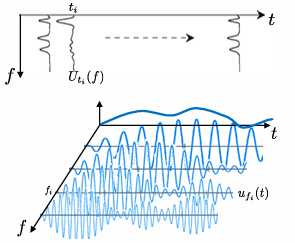
\includegraphics[width=0.3\linewidth]{images/filterbanksvsstftf.png}
\end{figure}

Modulating $h_0(n)$ by a carrier signal $e^{j 2 \pi f_k n T} = e^{j 2 \pi (k \frac{F_s}{N}) n T} = e^{j 2 \pi (k \frac{1}{NT}) n T} = e^{j 2 \pi \frac{kn}{N}}$ corresponds to shifting its frequency response by $f = f_k$ (center frequency of the $k$-th filter)
\begin{figure}[H]
    \centering
    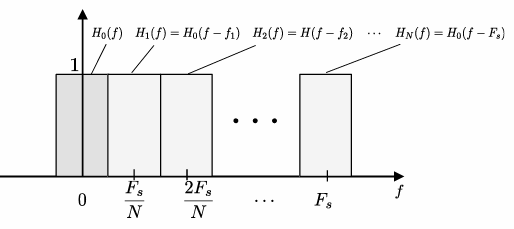
\includegraphics[width=0.5\linewidth]{images/filterbanksstuff.png}
\end{figure}

It is through this modulation process that we build a filterbank and partition the spectrum into subbands.
The rate of the outputs can be reduced $M$ times with no loss of information (in case of ideal frequency partition)
\begin{figure}[H]
    \centering
    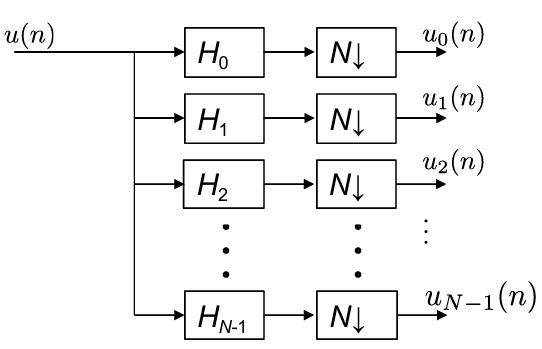
\includegraphics[width=0.5\linewidth]{images/filterbanksstff2.png}
\end{figure}

\subsubsection{STFT Frame by frame processing}
STFT is implemented (and normally interpreted) as a frame-by-frame Fourier Transform.

Each frame is obtained by applying a time-shifted window $w_m(n) = w(n - m)$ to select a portion of the signal $x(n)$ near time $m$.
We then compute the FFT of the windowed data to obtain the spectrum of the $m^{\text{th}}$ frame
\begin{figure}[H]
    \centering
    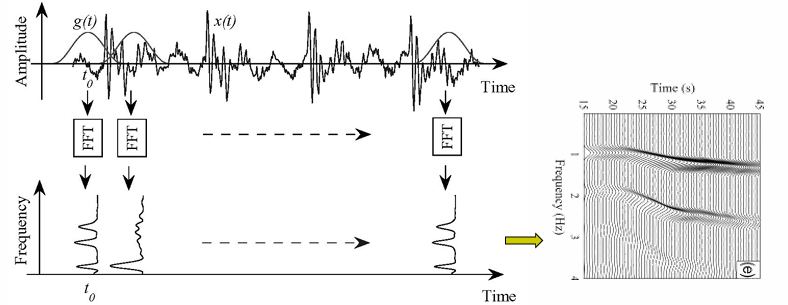
\includegraphics[width=0.75\linewidth]{images/stftstuff.png}
\end{figure}

Analysis:
\[x(nT) \xrightarrow{\text{STFT}} X(t_i, f_k) = \sum_{n} w_a(n) x(t_i + nT) e^{-j 2 \pi f_k n T}\]
\[X_{t_i}(f_k) = \sum_{n} w_a(n) x(i \alpha_a M_a T + nT) e^{-j 2 \pi \frac{kn}{N}}\]
where $w_a(n)$ is the analysis window, $\alpha_a$ the corresponding overlapping factor and $M_a$ its length (in samples), $i$ is the frame index, $N$ is the DFT size and $k$ is the index of the frequency bin $f_k = \frac{k}{TN}$.

The spectrum of a frame is here obtained by computing the FFT of a windowed signal, whose initial sample starts with the window (no linear phase accounting for a
shifting window). This is done by “shifting the signal back to the origin”.

Synthesis:
\[X(t_i, f_k) \xrightarrow{\text{ISTFT}} \tilde{x}(nT)  = \sum_{n} w_s(n - t_l) \frac{1}{N} \sum_{k=0}^{N-1}X(t_l, f_k) e^{j 2 \pi f_k nT}\]
\[\tilde{x}(nT)  = \sum_{n} w_s(n - l \alpha_s M_s) \frac{1}{N} 
\sum_{k=0}^{N-1}X(l \alpha_s M_s T, \frac{k}{NT}) e^{j 2 \pi \frac{kn}{N}}\]
where $w_s(n)$ is the synthesis window, $\alpha_s$ the corresponding overlapping factor and $M_s$ its length (in 
samples), $l$ is the frame index, $N$ is the DFT size and $k$ is the index of the frequency bin.


In Overlap and Add (OLA) processing we are  basically implementing a filterbank where the filters are a translated version of the Fourier transform of the window itself.
This is why temporal and frequency resolution are so linked to each other.
\begin{figure}[H]
    \centering
    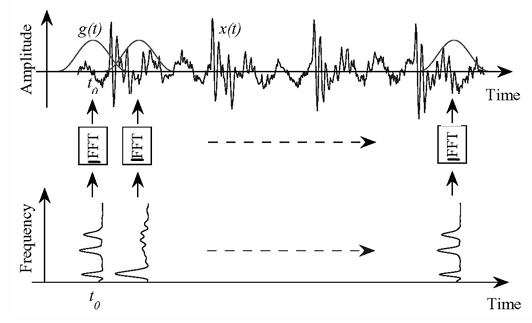
\includegraphics[width=0.65\linewidth]{images/ola2.png}
\end{figure}

Using a "slimmer" notation:
\[x(nT) \xrightarrow{\text{STFT}} X(t_i, f_k) = \sum_{n} w_a(n)x(t_i + nT)e^{-j2\pi f_k nT}\]

$\begin{aligned}
X_m(f_k) &= \sum_{n=-\infty}^{\infty} w(n)x(m + n)e^{-j2\pi f_k n N} , \quad m = i\alpha_a M_a \\
&= \sum_{r=-\infty}^{\infty} w(r - m)x(r)e^{-j2\pi f_k(r-m)N} , \quad r \triangleq m + n \to n = r - m \\
&= \sum_{r=-\infty}^{\infty} w(m - r)x(r)e^{j2\pi f_k(m-r)N} \quad \text{(even window)} \\
&= \sum_{r=-\infty}^{\infty} w_{f_k}(m - r)x(r) = w_{f_k} * x(m) , \quad w_{f_k}(m) \xrightarrow{\mathcal{F}} W(f - f_k)
\end{aligned}$

$X_m$ is the DTFT of the windowed signal (window starting from sample m). 
If we squeeze one domain, the other stretches. Its a constant area operation.
\begin{figure}[H]
    \centering
    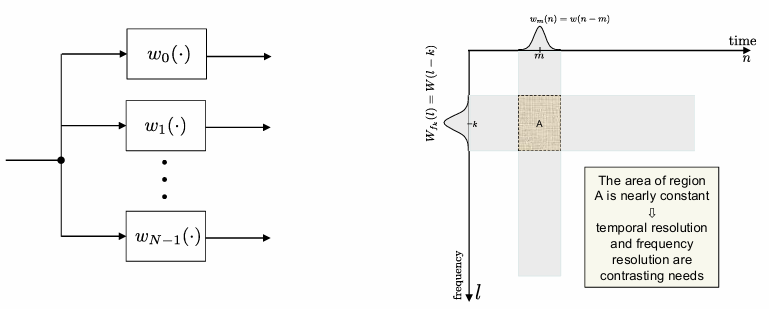
\includegraphics[width=0.85\linewidth]{images/filteerbankview.png}
\end{figure}

\clearpage
